%%%%%%%%%%%%%%%%%%%%%%%%%%%%%%%%%%%%%%%%%%%%%%%%%%%%%%%%%%%%%%%%%%%%%%%%%%%%%%%%%%%
\chapter{Unit-Tests}
\section{Ziel und Aufbau der Tests}
Ziel unserer Tests war nicht die vollständige Abdeckung aller Programmteile, sondern das exemplarische Aufzeigen, wie Unit-Tests im Rahmen einer
sauberen Architektur sinnvoll eingesetzt werden können. Im Mittelpunkt standen daher ausgewählte, fachlich relevante Methoden und Use Cases.

Wir haben uns darauf konzentriert, die Logik in der Domain- und Application-Schicht zu testen. Die Tests wurden mit xUnit geschrieben und folgen
durchgehend dem Arrange-Act-Assert-Muster.

Insgesamt wurden 11 Unit-Tests erstellt. Diese decken zentrale Bereiche der Domain- und Application-Schicht ab:

\begin{itemize}
    \item CareTaskTests: Fälligkeitsprüfung bei wiederkehrenden Aufgaben
    \item LocationTests: Validierung und Anlage von Standorten
    \item PlantTests: Erstellung und Aktualisierung von Pflanzen
\end{itemize}

Von 11 Tests waren 8 auf anhieb erfolgreich. Debei viel auf das besonders fehlerhafte Eingaben wie leere Strings in usecases und Konstrucktoren nicht
beachtet wurden.

\begin{figure}[H]
\centering
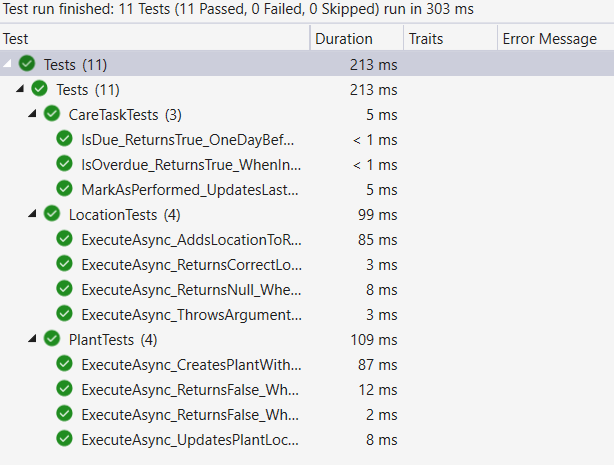
\includegraphics[width=0.50\textwidth]{img/tests.png}
\caption{Erfolgreicher Test-Durchlauf}
\end{figure}

\section{Einsatz von Mocks}
Um Use Cases isoliert zu testen, kamen Mocks zum Einsatz – erstellt mit dem Framework Moq. So konnten Repository-Interfaces ersetzt und typische
Szenarien simuliert werden wie etwa eine Abfrage, die ein bestimmtes Domain-Objekt zurückliefert oder die Prüfung, ob ein AddAsync-Aufruf mit
den erwarteten Daten erfolgt. Die Mocks ermöglichen saubere Unit-Tests ohne externe Infrastruktur.

Die Implementierungen der Repositories selbst wurden nicht getestet, da diese als Integrationstests zu werten wären und nicht zum Fokus eines Programmentwurfs im Sinne der Clean Architecture gehören.

\section{Teststrategie und Abdeckung}
Die Testabdeckung wurde mit Coverlet gemessen. Der Gesamtwert beträgt 15,3 \%, was angesichts der gezielten Auswahl und des prototypischen Charakters des Projekts erwartbar war.
Es wurden nur sehr wenige kleine Aspekte der Anwendung getestet. Komplexe Controller sind nicht implementiert und konnten daher auch nicht getestet werden.

Viele Zeilen entfallen zudem auf DTOs, Konfigurationen oder technische Infrastruktur (z. B. Datenbankadapter).

\begin{figure}[H]
\centering
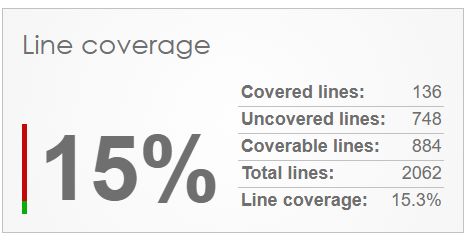
\includegraphics[width=0.50\textwidth]{img/coverage.png}
\caption{Coverrage durch Unit-Tests}
\end{figure}

Die Tests dienten dabei auch zur Reflektion der Architektur: Wiederverwendbarkeit, Testbarkeit und Trennung von Zuständigkeiten. Sie helfen den Entwicklungsprozess aktiv zu hinterfragten und zu verbessern.

\section{ATRIP-Analyse}
Unsere Tests erfüllen die ATRIP-Kriterien im Rahmen des Programmentwurfs in sinnvoller Weise.

\begin{itemize}
    \item Automatic: Alle Tests sind vollständig automatisiert mit xUnit eingebunden. Sie lassen sich ohne manuelle Schritte per dotnet test ausführen.
Auch die Code Coverage wurde über Coverlet integriert, was den automatisierten Testprozess sinnvoll ergänzt.
    \item Thorough: Wir haben nicht alle relevanten Funktionen getestet – insbesondere Randfälle, Validierungslogik und Fehlerbehandlung wurden
größtenteils ausgespart. Das war allerdings eine bewusste Entscheidung. Stattdessen haben wir exemplarisch zentrale fachliche Methoden getestet,
z. B. die Fälligkeitsprüfung bei Pflegeaufgaben oder das Erstellen und Aktualisieren von Pflanzen. Die Tests zeigen, dass unser Code testbar
aufgebaut ist, auch wenn nicht alle Fälle abgedeckt sind.
    \item Repeatable: Alle Tests laufen stabil und liefern reproduzierbare Ergebnisse. Es gibt keine externe Abhängigkeit (z. B. Datenbank), weil alle
Infrastrukturkomponenten gemockt wurden. Ein Beispiel ist CreatePlant, bei dem das Repository vollständig isoliert und das Verhalten überprüfbar
ist.
    \item Independent: Unsere Tests sind voneinander unabhängig. Jeder Test initialisiert seine eigene Datenbasis, es gibt keine gemeinsame Setup-Logik
oder globale Zustände. Das gilt sowohl für einfache Domain-Methoden als auch für die Use Cases.
    \item Professional: Die Tests sind klar benannt und strukturiert. Wir folgen durchgängig dem AAA-Muster.
\end{itemize}

\begin{figure}[H]
\centering
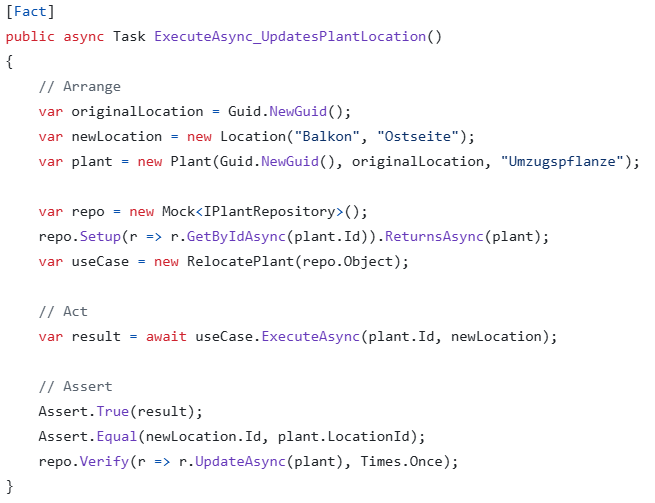
\includegraphics[width=1.00\textwidth]{img/test.png}
\caption{Beispiel für einen Test}
\end{figure}